\documentclass{beamer}
\def \sarccontrib {{\bf SARC contribution}}
\begin{document}
\title{Optimizing the software stack of a cosmic proportions cluster of multi-core machines}
\author{Sebastian Pop}
\institute{SARC: Samsung Austin R\&D Center}
\date{February 5, 2017}

\frame{\titlepage}

\frame{\frametitle{Android: a cosmic size cluster}
  \begin{itemize}
  \item top500: $10M$ cores / $15.3MW$ \footnote{\url{https://www.top500.org/lists/2016/11}} / US$\$273$ million \footnote{\url{https://en.wikipedia.org/wiki/Sunway_TaihuLight}}
  \item Android devices: $\sim{}6B$ cores \footnote{4 cores / device} / $\sim{}300MW$ \footnote{battery $13.2Wh = 4.4V * 3000 mAh$, charging every 48 hours} / $\sim{}$US\$0
  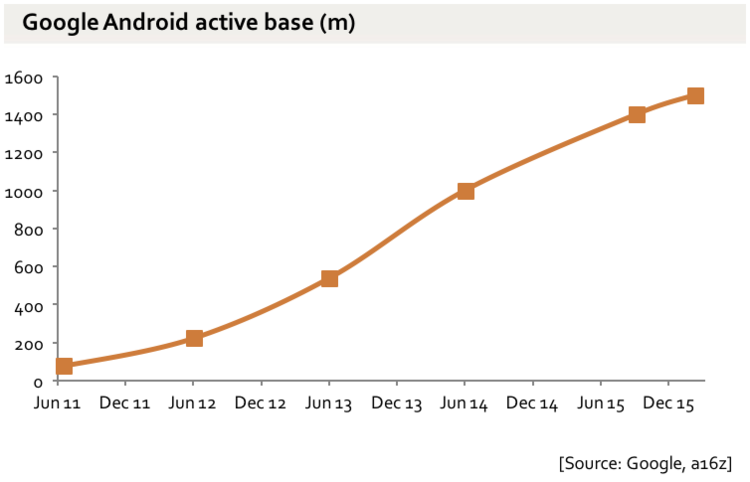
\includegraphics[width=8cm]{active-devices.png}
  \end{itemize}
}

\frame{\frametitle{Android Open Source Project (AOSP) Software Stack}
  \begin{itemize}
  \item<1-> AOSP: common base for Android devices (+ customizations)
  \item<1-> C/C++ for the platform libraries, Java for user interface
    {\small \begin{tabular}{c c c}
      ansic & 22 MLoC & 39\% \\
      cpp   & 13 MLoC & 23\% \\
      java  & 10 MLoC & 17\% \\
    \end{tabular}}
  \item<1-> $\sim80\%$ execution cycles in C/C++, $\sim20\%$ in Java
  \item<2-> release/updates/deprecation ($5\sim6$ years) \\
    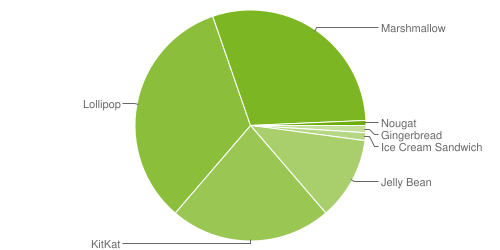
\includegraphics[width=8cm]{android-versions.png} \footnote{Data collected during a 7-day period ending on January 9, 2017.}
  \end{itemize}
}

\frame{\frametitle{Why Optimizing the Performance of Android?}
  \onslide<1-> {
    \begin{itemize}
    \item the code of Android is cold (flat profile), full of branches
    \item there are few loops (image processing, compression, etc.)
    \end{itemize}
  }
  \vspace{.3cm}
  \onslide<2-> {
    Overall picture:
    \begin{itemize}
    \item same code executed billions of time
    \item outer loop is outside the device
    \item profile how often code is in use
    \item variation over time following popularity of apps
    \item continuously monitor usage patterns
    \item tune code optimziations over time
    \end{itemize}
    \vspace{.3cm}
    \begin{tabular}{c c c}
      $\$0.30$ / device / year & $\longrightarrow$ & $\$300M$ / billion devices / year \footnote{$\$0.12/kWh$, battery $13.2Wh = 4.4V * 3000 mAh$, charging every 48 hours} \\
      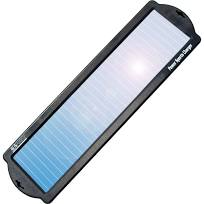
\includegraphics[width=1.5cm]{1watt.jpg} & & 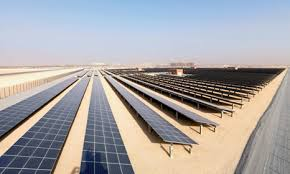
\includegraphics[width=3cm]{1GWatt.jpg}
    \end{tabular}
  }
}

\frame{\frametitle{Agenda}
  \begin{itemize}
  \item Performance analysis: hot spots
  \item Improve performance of AOSP libraries
  \item Enable continuous profiling and optimizations (AutoFDO)
  \item Enable more secure execution environment (CFI)
  \end{itemize}
}

\frame{\frametitle{Performance Analysis}
  \begin{itemize}
  \item benchmarks: track performance over time (compiler/libraries)
  \item linux perf: profile of cycles (per function, hot-spots)
  \item valgrind: number of executed instructions (branches, R/W)
  \item static profiles: how many uses for a function
  \end{itemize}
}

\frame{\frametitle{Benchmarks}
  track performance over time (compiler/libraries) \\
  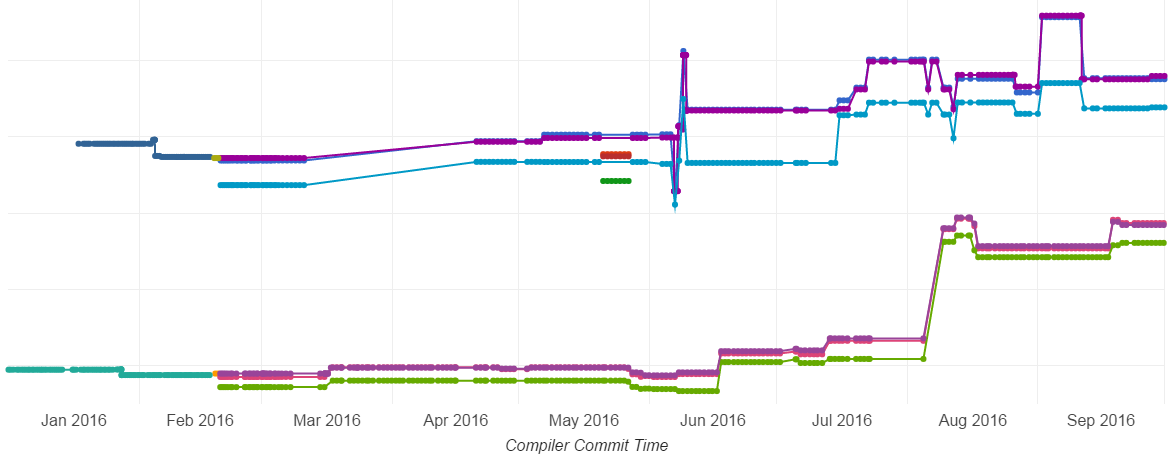
\includegraphics[width=11cm]{benchmarks.png}  
}

\frame{\frametitle{Benchmarks}
  on a real device (and a noisy benchmark...)
  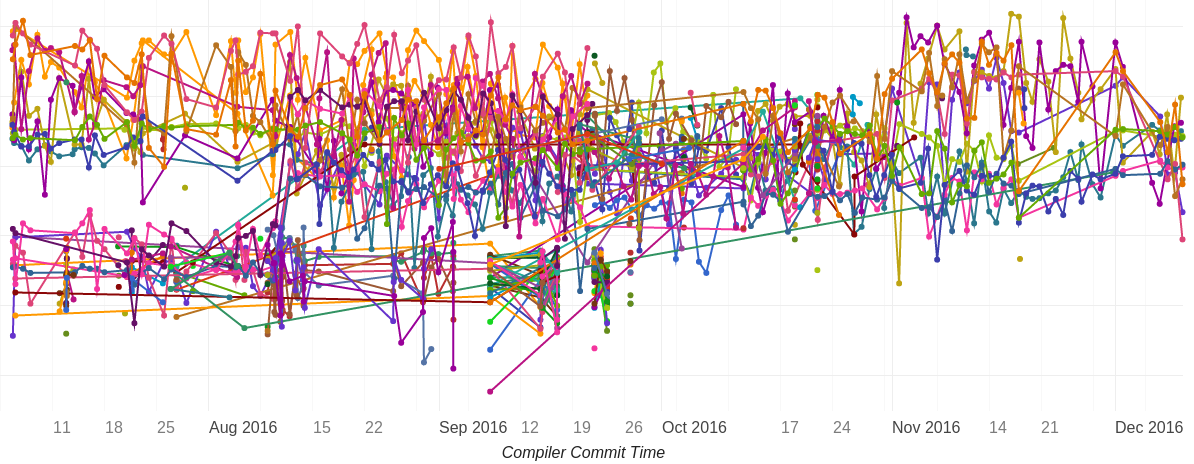
\includegraphics[width=11cm]{benchmarks-device.png}  
}

\frame{\frametitle{Linux Perf}
  
}

\frame{\frametitle{Valgrind}
  
}

\frame{\frametitle{Static Profile}
  
}

\frame{\frametitle{Improve performance of libraries}
  \begin{itemize}
  \item \sarccontrib{}: std-benchmark\footnote{https://github.com/hiraditya/std-benchmark}
  \item std-benchmark provides micro-benchmarks for each function in C/C++ standard libraries
  \item detect room for improvement
    \begin{itemize}
    \item compile with different compilers
    \item link with different standard libraries
    \item run on different machines: CPUs, architectures
    \end{itemize}
  \item 
  \end{itemize}
}

\frame{\frametitle{AutoFDO: Feedback Directed Optimization}
  \begin{itemize}
  \item linux-perf extracts profiles of running systems
  \item little to no overhead \footnote{Google Wide Profiling: A Continuous Profiling Infrastructure for Data Centers, IEEE Micro (2010)}
  \item compute basic block frequencies from profiles
  \item better inlining \footnote{Lightweight Feedback-Directed Cross-Module Optimization, CGO 2010}
  \item hot/cold code placement, register allocation, jump-threading
  \item Intel-LBR (last branch record): last 16 taken branches
  \item provides precise basic block execution frequency
  \item how do we do this on ARM?
  \end{itemize}
}

\frame{\frametitle{ARM-ETM: Embedded Trace Macrocell}
  \begin{itemize}
  \item ARM-ETM: records execution traces (for debug)
  \item dedicated circular buffer 1 to 3MB ($\sim10^5$ branches/MB)
  \item no overhead
  \item support in Linux kernel by Mathieu Poirier (Linaro)
  \item next android kernel linux-4.9 will support ARM-ETM
  \item \sarccontrib{:} how to use ARM-ETM for AutoFDO
    \begin{itemize}
    \item perf-inject translates execution traces to LBR events
    \item patch similar to perf-inject for Intel Process Trace
    \end{itemize}
  \end{itemize}
}

\frame{\frametitle{From Profiles to Power Usage}
  \begin{itemize}
  \item  \footnote{An Analysis of Power Consumption in a Smartphone, USENIX'10}
  \end{itemize}
}

\frame{\frametitle{Towards more secure devices}
  \begin{itemize}
  \item Control Flow Integrity (CFI): $2\%$ overhead \footnote{Enforcing Forward-Edge Control-Flow Integrity in GCC\&LLVM, USENIX'14}
  \item to enable on Android: need to further reduce its cost
  \end{itemize}
}

\end{document}
